%This document is a preview lecture for college class: Mathematical History.
%I'm a student majoring in Mathematics in China university.
%This article must has lots of shortcomings, and I sincerely invite collegues and friends to criticize, correct it.

\documentclass{Math_Note}

\title{Mathematical History(CN)}
\author{Buce-Ithon}
\newdateformat{mydate}{\twodigit{\THEDAY}{ }\shortmonthname[\THEMONTH], \THEYEAR}
\date{\today}

\begin{document}

%Title page
\maketitle

%content
\newpage
\tableofcontents
\newpage

%Chapter 1
\section{数学史——人类文明史的重要篇章}
数学史研究数学概念、数学方法和数学思想的起源和发展,及其与社会、政治、经济和一般文化的联系.
\subsection{数学史的意义}
数学作为一门发展历程几乎贯穿了人类发展史的学科,其历史性或者说积累性极强,在人类整个文明史上有着特殊的地位.
这种地位,是由数学作为一种文化的特点决定的:
\begin{itemize}
    \item 抽象性(追求高的精确、可靠的知识)
    \item 一般性(追求世界规则最大限度的一般性模式的倾向)
    \item 创造性(艺术特色)
\end{itemize}
数学是各个时代人类文明的标志之一,是了解整个人类文明史的重要渠道.
\subsection{什么是数学——历史的理解}
古希腊哲学家亚里士多德:“数学是量的科学”.

恩格斯:“数学是研究现实世界的空间形式与数量关系的科学”.

前苏联数学家:“现代数学就是各种量之间的可能的,一般说是各种变化着的量的关系与相互联系的数学”.

20世纪80年代开始,一批美国学者:“数学这个领域已被称作模式的科学(science of pattern),其目的是要解释人们从自然界和数学本身的抽象世界中所观察到的结构和对称性”.
\subsection{关于数学史的分期}
通常来说,数学史的分期线索如下:
\begin{itemize}
    \item 按时代顺序
    \item 按数学对象、方法等本身的质变过程
    \item 按数学发展的社会背景
\end{itemize}

本书(《数学史概论》)综合上述线索,作出数学史的如下分期:
\begin{enumerate}
    \item 数学的起源与早期发展 (公元前 6 世纪前)
    \item 初等数学时期 (公元前 6 世纪–16 世纪)
    \begin{enumerate}
        \item 古代希腊数学 (公元前 6 世纪–6 世纪)
        \item 中世纪东方数学 (3 世纪–15 世纪)
        \item 欧洲文艺复兴时期 (15 世纪–16 世纪)
    \end{enumerate}
    \item 近代数学时期 (或称变量数学建立时期, 17 世纪–18 世纪)
    \item 现代数学时期 (1820'–现在)
    \begin{enumerate}
        \item 现代数学酝酿时期 (1820'-1870')
        \item 现代数学形成时期 (1870'-1940')
        \item 现代数学繁荣时期 (或称当代数学时期, 1950'–现在)
    \end{enumerate}
\end{enumerate}

%Chapter 2
\section{数学的起源与早期发展}
\subsection{数与形概念的产生}
\subsubsection{初等算术}
早期人类识别事物多寡的能力促进了抽象的“数”的概念的产生。而“数”的诞生也促成了计数的需求和发展.

计数历史:手指计数$\rightarrow$石子计数$\rightarrow$结绳计数、刻痕计数$\rightarrow$书写计数与计数系统

计数系统:古埃及的象形数字(公元前3400年左右),巴比伦楔形数字(公元前2400年左右),中国甲骨文数字(公元前1600年左右),
希腊阿提卡数字(公元前500年左右),中国筹算数码(公元前500年左右),印度婆罗门数字(公元前300年左右),玛雅数字(?)

其中,除巴比伦楔形数字采用六十进制、玛雅数字采用二十进制以外,其他均属十进制数系.

\subsubsection{初等几何}
与算术相仿,最初的几何知识是从人们对形的直觉中萌发出来的.

\begin{itemize}
    \item 古希腊学者希罗多德(Herodotus, 约公元前484~前425)研究:古埃及几何学的起源产生于尼罗河泛滥后土地的重新测量. 
    “几何学”一词的希腊文γεωμετρία意即“测地”.
    \item 古代印度几何学的起源则与宗教实践密切相关:公元前8世纪至公元前5世纪形成的所谓“绳法经”,
    记载了关于祭坛和寺庙建造中的几何问题和求解法则.
    \item 古代中国:几何学更多地与天文观测相联系,流传下来的经典著作有《周髀算经》、《九章算术》(后者多被认为是中国古代算术经典)等.
\end{itemize}

\subsection{河谷文明和早期数学}
历史学家往往把兴起于埃及、美索不达米亚、中国和印度等地域的古代文明称为“ 河谷文明”.
\subsubsection{埃及数学}
埃及象形文字(hieroglyphic, 意为“ 圣刻”——神圣的雕刻)产生于公元前3500年左右,约公元前2500 年被简化为一种更易书写的“僧侣文 ”(hieratic) ,后又发展成所谓“通俗文 ”(domotic).

古埃及人在一种用纸莎草(Papyrus)压制成的草片上书写,这些纸草书有的幸存至今. 关于古埃区数学的知识,主要就是依据了两部用僧侣文写就的纸草书——莱茵德纸草书和莫斯科纸草书. 

(有趣的是,两部纸草书虽然均出自于埃及,然而由于历史原因,均流传到国外,最终以埃及以外的其他地区命名)

两部纸草书实际上都是各种类型的数学问题集:莱茵德纸草书主体由84个问题组成,莫斯科纸草书包括了25个问题.

此外,埃及人很早就发明了象形文字记号,这是一种以十进制为位值的系统,但却没有进位的概念. 这种计数制用不同的特殊记号分别表示10的前六次幂. 如下图所示:

\begin{figure}[H]
    \centering
    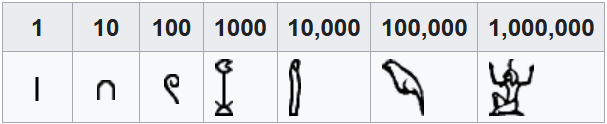
\includegraphics[scale=0.8]{"./Figures/Ancient_Egyptian_Math_1.png"} %[scale=xxx]-->[height=xxx, width=xxx]
    \caption{古埃及计数系统-10的幂次}
\end{figure}
\begin{figure}[H]
    \centering
    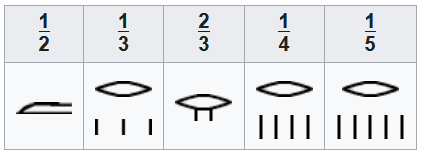
\includegraphics[scale=0.8]{"./Figures/Ancient_Egyptian_Math_2.png"}
    \caption{古埃及计数系统-分数}
\end{figure}

\end{document}
